\documentclass{article}
\usepackage[utf8]{inputenc}
\usepackage[spanish]{babel}
\usepackage{graphicx, graphics, float, fancyhdr, titling}
\usepackage{listings}
\usepackage[a4paper, total={6in, 9.5in}]{geometry}
\usepackage{fancyhdr}
\usepackage{hyperref}   %para que funcione addcontentsline debe ser la ultima que se cargue

%\setcounter{secnumdepth}{-2}       %Poner solo esto si no se quieren numero delante de las secciones y niveles inferiores.

\renewcommand{\footrulewidth}{0.4pt}
\title{

\includegraphics[width=1.75in]{imagenes/UGR-Logo.png} \\
\vspace*{1in}
\textbf{Cuestiones Tema 2} \\
Animación por Ordenador \\
\vspace*{0.5in}}
\author{Andrés Merlo Trujillo \\
andresmerlo@correo.ugr.es \\
77147239H \\ 
\vspace*{0.5in} \\
E.T.S. de Ingenierías Informática y de Telecomunicación \\
\textbf{Universidad de Granada}} \date{\today}

\hypersetup{
    colorlinks=true,
    linkcolor=black,
}

\renewcommand\maketitlehooka{\null\mbox{}\vfill}
\renewcommand\maketitlehookd{\vfill\null}

\begin{document}
\begin{titlingpage}
\maketitle
\end{titlingpage}

\tableofcontents

\newpage

\pagestyle{fancy}   %a partir de comienza el header (se salta el indice y portada)
\fancyhead[L]{Andrés Merlo Trujillo}
\fancyhead[R]{Animación por Ordenador}
%\section{Ejercicio 1}
%\begin{figure}[H]
%    \centering
%    \includegraphics[width=\textwidth]{imagenes/passwdfile.png}
%\end{figure}

\section{Busca el resto de principios de animación, descríbelos brevemente e indica un ejemplo visual de cada uno.}

Voy a explicar cada uno de los principios en subsecciones a continuación.

% overlap: meh

\subsection{Overlap \& Follow Through}

Son dos técnicas que se utilizan con el objetivo de crear una animación más realista y para dar la sensación de que el personaje tiene una inercia [https://www.brownbagfilms.com/labs/entry/12-principles-of-animation-follow-through-and-overlapping-action-tutorials]. La idea principal de estas técnicas las partes secundarias de un personaje se mueven a un ritmo diferente del personaje durante el movimiento del mismo y mantienen una inercia cuando el personjae se para.

\bigskip

\textit{Follow Through} se basa en la idea en que ciertas partes conectadas a un personaje/objeto se seguirán moviendo después de que dicho objeto haya parado [https://www.brownbagfilms.com/labs/entry/12-principles-of-animation-follow-through-and-overlapping-action-tutorials].

\bigskip

Mientras que el \textit{Overlapping} se basa en la idea en que las partes conectadas a un personaje/objeto se moverán a un ritmo diferente del mismo [https://www.brownbagfilms.com/labs/entry/12-principles-of-animation-follow-through-and-overlapping-action-tutorials], normalmente en el sentido contrario en el que se mueven el personaje, para dar sensación de velocidad.

\bigskip

Ejemplos de este principio pueden ser: movimientos de brazos de un personaje, movimiento de las orejas de un animal que correo y luego para, o incluso el movimiento de una antena de un personaje.

\begin{figure}[H]
    \centering
    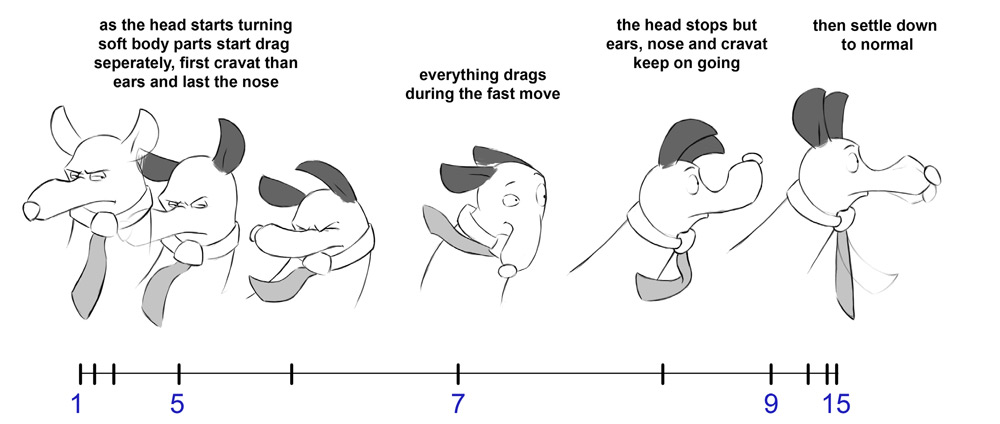
\includegraphics[width=\textwidth]{imagenes/overlap-08.jpg}
    \caption{Ejemplo del principio de \textit{Overlapping} y \textit{Follow Through}. Se puede ver en las orejas y la corbata.}
    \caption{Enalce: https://www.robert-kuczera.de/3d-character-animation-tutorial-secondary-actoin.html}
\end{figure}

\subsection{Slow-in \& Slow-out}

% Este principio consiste en que los objetos cuando se mueven en la vida real no lo hacen de manera abrupta, sino acelerando para comenzar a moverse y decelerando cuando se van a parar. 

Este principio consiste en hacer que un objeto acelere cuando vaya a comenzar a moverse y decelere cuando se vaya a parar. Esto se hace de esta forma porque en la vida real los objetos no se mueven sin antes acelerar o decelerar. Realizar una animación sin este principio puede hacer que los movimientos parezcan naturales, robóticos y abruptos. [https://www.pluralsight.com/blog/film-games/understanding-12-principles-animation]

\bigskip

Un ejemplo de este principio es en un coche que sale de parado y luego frena de nuevo, el coche necesita un tiempo para llegar a la velocidad deseada; es decir, una aceleracion. Luego cuando frena pasa exactamente lo mismo, no para bruscamente, sino que va decelerando poco a poco. [https://www.pluralsight.com/blog/film-games/understanding-12-principles-animation]

\bigskip

En animación tradicional, esto se realiza haciendo uso de espaciados: en el comienzo y final de la animación se dibujan más fotogramas seguidos, mientras que en el resto se mantiene un espaciado mayor, pero constante, para que el resultado final sea el correcto [https://www.pluralsight.com/blog/film-games/understanding-12-principles-animation]. El espaciado menor producirá que se le dedique más tiempo (fotogramas) a la animación, mientras que el mayor menos, haciendo que se de dicha sensación.

\bigskip

En la animación por ordenador, normalmente se suele hacer con una curva \textit{Ease-In/Ease-Out}, que realiza exactamente lo mismo que con las aniamciones tradicionales, pero automaticamente.

\begin{figure}[H]
    \centering
    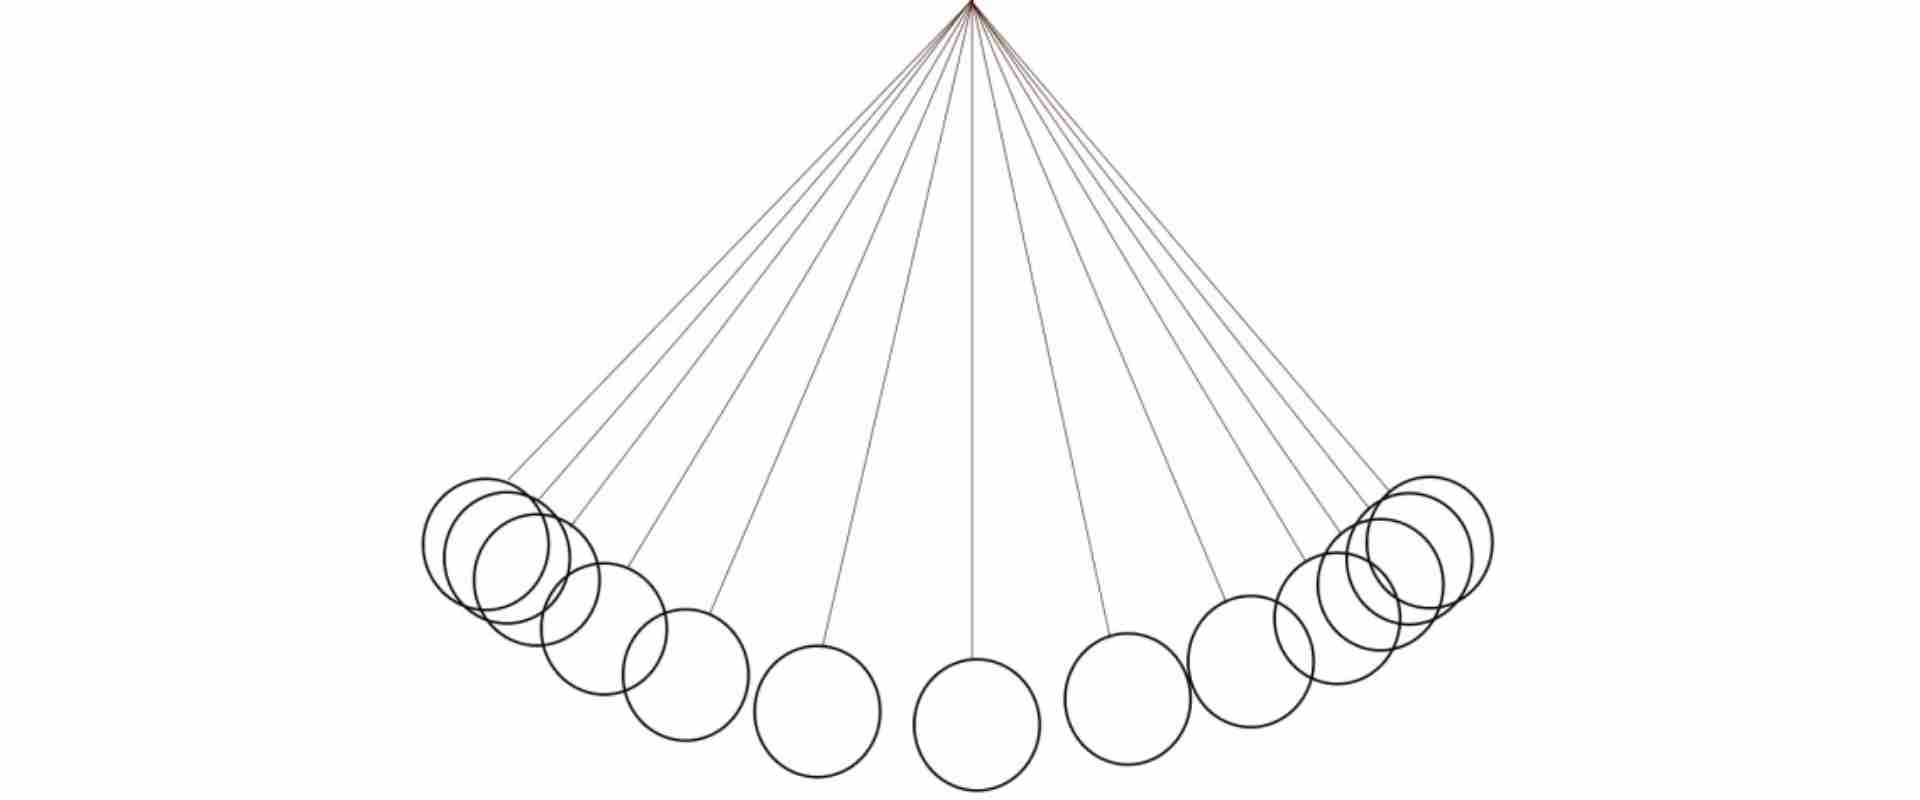
\includegraphics[width=\textwidth]{imagenes/Slow-In-and-Slow-Out.jpg}
    \caption{Ejemplo del principio \textit{Slow-In \& Slow-Out}. Se puede ver como el péndulo en los extremos acelera y decelera mediante el espaciado de los fotogramas.}
    \caption{Enalce: https://darvideo.tv/dictionary/slow-in-slow-out/}
\end{figure}
\end{document}
